\documentclass[12pt,a4paper]{article}

\usepackage[a4paper, top = 2cm, bottom = 2cm, left = 1.5cm, right = 1.5cm]{geometry}
\usepackage[dvipsnames]{xcolor} % Colors

\usepackage{standalone}

\usepackage{setspace}
\usepackage{graphicx}
\usepackage{amsfonts}
\usepackage{amsmath}
\usepackage{tikz}
\usepackage{pdfpages}
\usepackage{epigraph}
\usepackage{csquotes}
\usepackage{natbib}
% Bibliography
\usepackage{xcolor}
\usepackage{hyperref}
\hypersetup{
colorlinks=true,
citecolor=MidnightBlue,
linkcolor=MidnightBlue,
pdfpagemode=FullScreen}

\usepackage{listings}
\lstset{frame=tb,
  language=Matlab,
  aboveskip=3mm,
  belowskip=3mm,
  showstringspaces=false,
  columns=flexible,
  basicstyle={\small\ttfamily},
  numbers=none,
  numberstyle=\tiny\color{gray},
  keywordstyle=\color{Red},
  commentstyle=\color{MidnightBlue},
  stringstyle=\color{mauve},
  breaklines=true,
  breakatwhitespace=true,
  tabsize=3
}

\usepackage{natbib}
\usepackage[noabbrev]{cleveref}
\setcitestyle{authoryear,open={(},close={)}}
\bibliographystyle{plainnat}

\usepackage{subfiles}

\usepackage{url}
\urlstyle{same} % omit this command if you want monospaced-font look
\newcommand\purl[1]{\protect\url{#1}} % "protected url"

\setlength\parindent{0pt}
\spacing{1.2}

\begin{document}

\begin{center}
       \vspace*{4cm}
       \huge\textbf{Project 5} \\
       \vspace{0.4cm}
       \large \textbf{Public Finance in Macroeconomics} \\
       \vspace{0.5cm}
        \large Handed in by the \textcolor{orange}{\textbf{Heterogeneous Geeks}} \\
        \vspace{0.3cm}
        a.k.a. Vivien Voigt, Thong Nguyen, 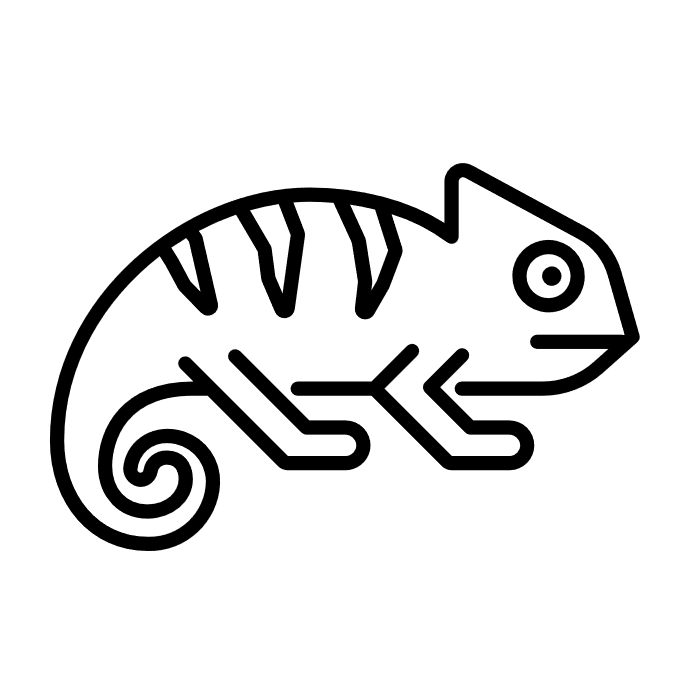
\includegraphics[scale=0.06]{geek.png}\\Davide Difino \& Celina Proffen \\
       \vspace{1.5cm}
       \vfill



        Project in the context of Prof. Ludwig's course: \\
        \textbf{Public Finance in Macroeconomics: Heterogenous Agent Models}\\
        at the Graduate School of Economics, Finance, and Management
       \vspace{0.8cm}
   \end{center}

\newpage

%-----------------------------------------------------

\section*{Problem 1: Solution}

\subsection*{Explain all sections of the code}

The code defines several functions for different purposes:

\begin{lstlisting}[frame=single]
% -------------------------------------------------------------------------------%
% use all functions below to print graphs
function towards_olg
% -------------------------------------------------------------------------------%

% -------------------------------------------------------------------------------%
% define the values of parameters
function func_calibr(opt_det,opt_nosr,opt_ny)
% ------------------------------------------------------------------------------- %

% ------------------------------------------------------------------------------- %
% solution of the household problem
%    prints:
%       - state variable matrix (gridx)
%       - saving grid (gridsav)
%       - optimal consumption function (cfun)
%       - optimal value function (vfun)
function [gridx,gridsav,gridass,cfun,vfun] = func_hh
% ------------------------------------------------------------------------------- %

% ------------------------------------------------------------------------------- %
% aggregation and cross-sectional measure
%   prints:
%       - distribution of assets conditional by age and shock (Phi)
%       - distribution of assets (PhiAss)
function [Phi,PhiAss,ass]=func_aggr(gridx,gridsav,cfun,gridass)
% ------------------------------------------------------------------------------- %

% ------------------------------------------------------------------------------- %
% compute average life-cycle profiles
function [labinclife,inclife,asslife,conslife,vallife] = lcprofile(Phi,gridass,cfun,vfun)
% ------------------------------------------------------------------------------- %

% ------------------------------------------------------------------------------- %
% utility function
function u = U(c)
% ------------------------------------------------------------------------------- %
\end{lstlisting}
\pagebreak
\begin{lstlisting}[frame=single]
% ------------------------------------------------------------------------------- %
% marginal utility function
function muc=MUc(c)
% ------------------------------------------------------------------------------- %

% ------------------------------------------------------------------------------- %
% construction of the Markov chain process
%   prints:
%       - transition matrix first eigenvector (pini)
%       - shocks values (gridy)
%       - transition matrix (pi)
function [pini,pi,gridy]=mchain(rhoeta,epsil)
% ------------------------------------------------------------------------------- %

% ------------------------------------------------------------------------------- %
% this function computes the inverted of the utility function
% it is required in func_hh to retrive optimal consumption from the value function
function invut=invut(marg)
% ------------------------------------------------------------------------------- %

% ------------------------------------------------------------------------------- %
% create curved grid using curvature parameter c
function grd = makegrid(x1,x2,n,c)
% ------------------------------------------------------------------------------- %
\end{lstlisting}

The function towards\_olg is the main function. It uses the calibration and calculations of the other functions to produce the following graphs:

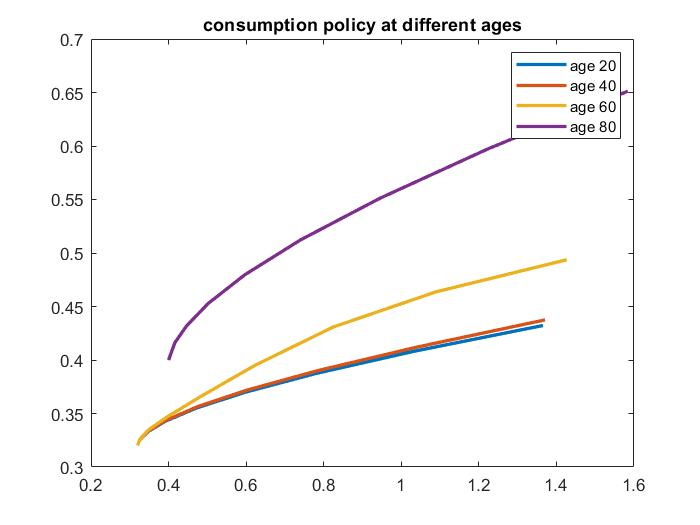
\includegraphics[width=14cm]{Graphs/Figure1} \\
This graph depicts the consumption policy at different ages. Thereby, the x-axis shows grid cash-on-hand gridx and the y-axis shows consumption. In general, we can observe that the level of consumption for every given grid cash-on-hand level is higher for older age groups, yet, consumption and grid cash-on-hand have a positive relation for all age groups. This shock state is held fix within this graph. \\
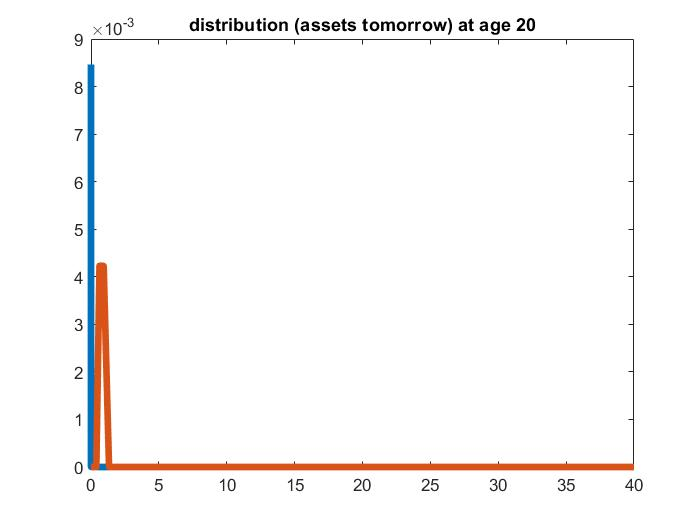
\includegraphics[width=14cm]{Graphs/Figure2} \\
This graph depicts the assets distribution at age 20. We can see that this distribution is dense. This is the case because age 20 individuals have just entered the labour market and, therefore, could not build up large savings. Question: What is blue? Assets today? What is red? Expected assets tomorrow? \\
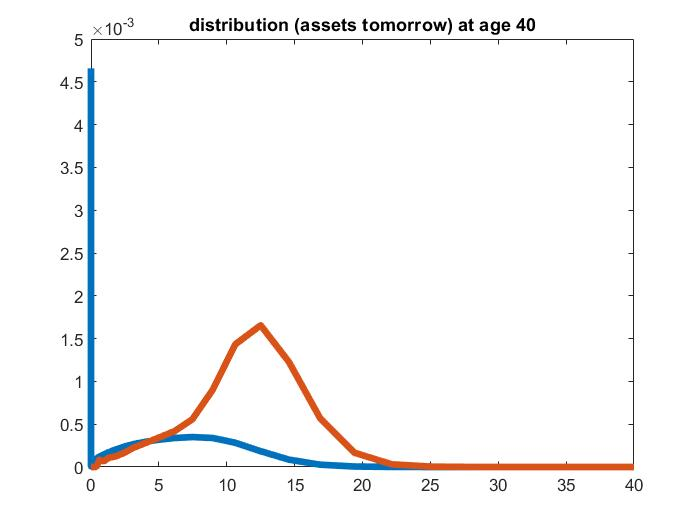
\includegraphics[width=14cm]{Graphs/Figure3} \\
This graph depicts the assets distribution at age 40. This distribution is less dense because age 40 individuals already had some time to accumulate wealth. \\
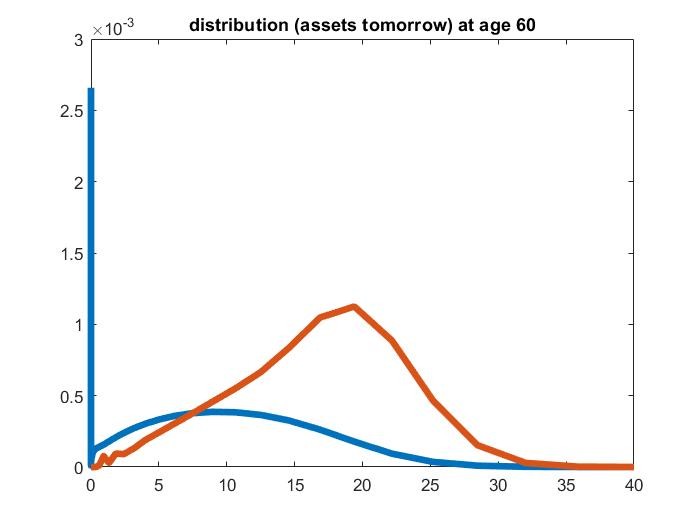
\includegraphics[width=14cm]{Graphs/Figure4} \\
This graph depicts the assets distribution at age 60.\\
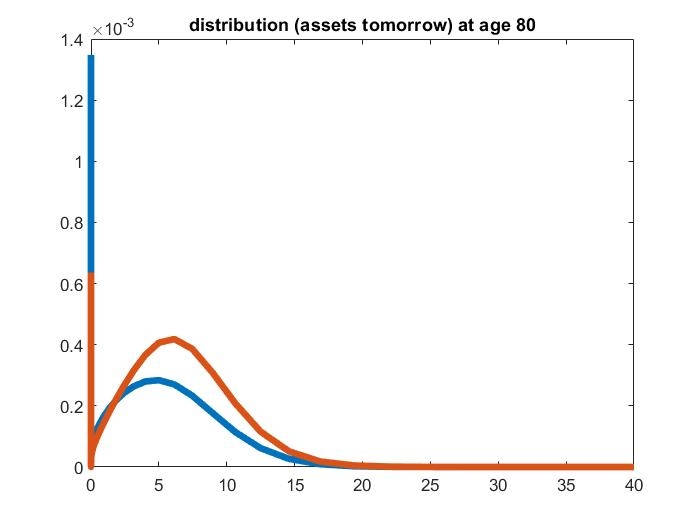
\includegraphics[width=14cm]{Graphs/Figure5} \\
This graph depicts the assets distribution at age 80. Since induviduals die for sure at age 100, both, the blue and the red line, are expected to be zero 20 years into the future.\\
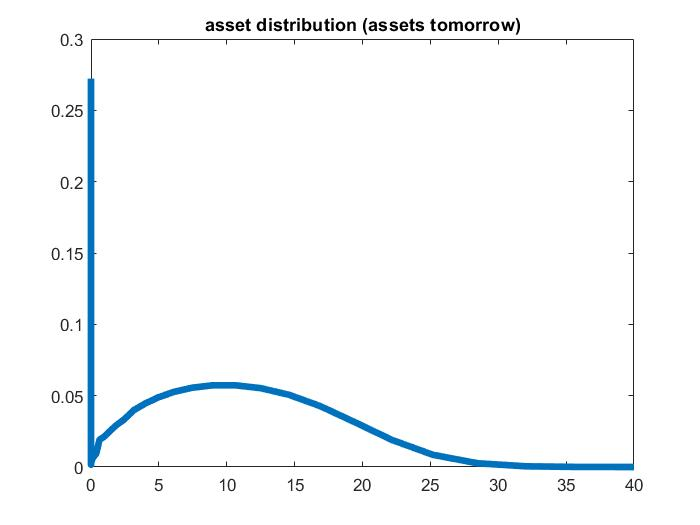
\includegraphics[width=14cm]{Graphs/Figure6} \\
This is an aggregate asset distribution. On average, that is over all age groups, assets are expected to increase and decrase again during each live span.\\
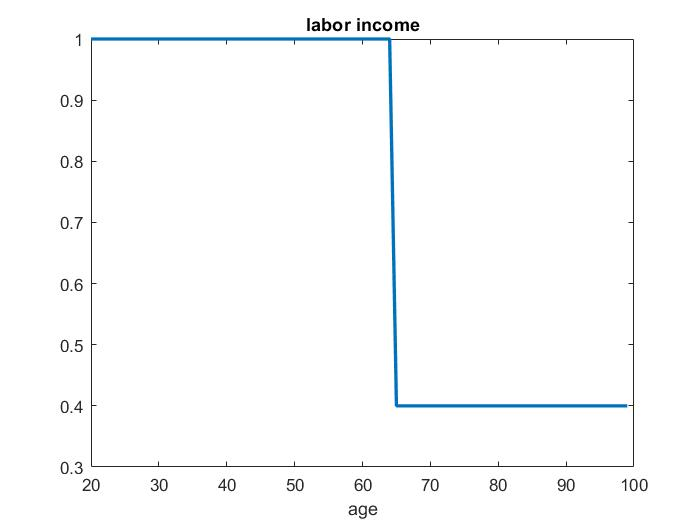
\includegraphics[width=14cm]{Graphs/Figure7} \\
This graph depicts an individual's labour income. The model is calibrated in a way that an individual earn the full wage (normalised to 1) between 20 and 65 years of age and receives a pension of 40\% of his/ her former income until his/ her death. Death occurs for sure at age 100.\\
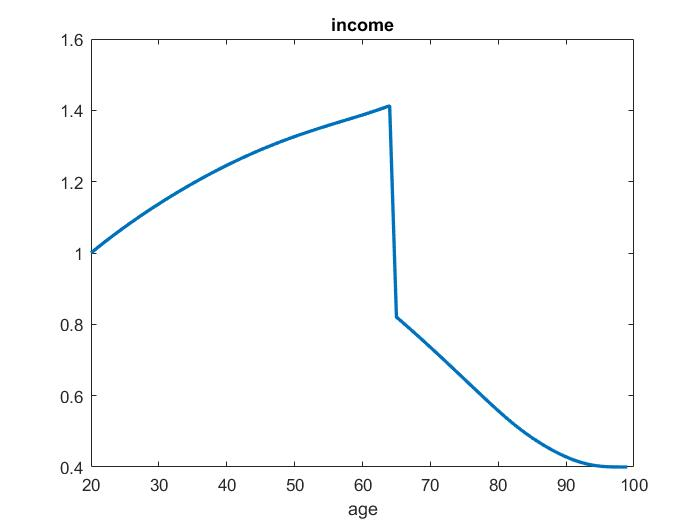
\includegraphics[width=14cm]{Graphs/Figure8} \\
This graph depicts overall income, that is labour income plus all other sorts of income (interest payment on savings). Overall income is rising until the retirement age (65) is reached. Afterwards the individual receives 40\% of his/ her former labour income plus interest payments for his/ her saving. Interest payments get smaller and smaller because the individual consumes part of his/ her savings in each period.\\
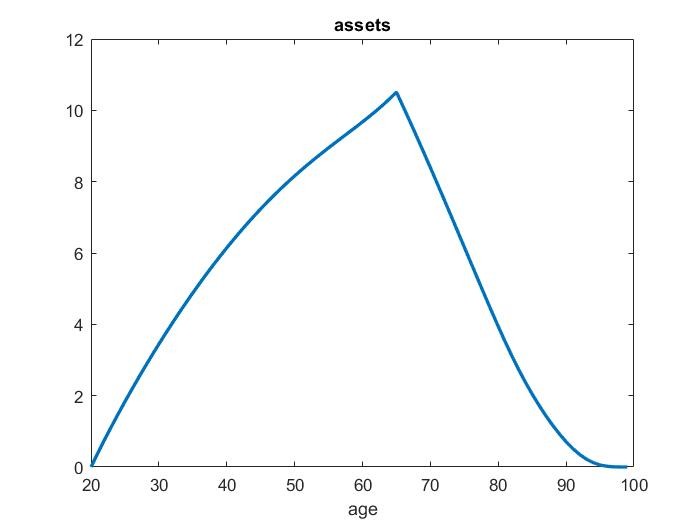
\includegraphics[width=14cm]{Graphs/Figure9} \\
This graph depicts the overall asset distribution over the life cycle. Assets reach a maximum at age 65 (retirement age) and afterwards decrease until death. If an induvidual reaches the maximum age of 100 years, his/ her assets are fully consumed. \\
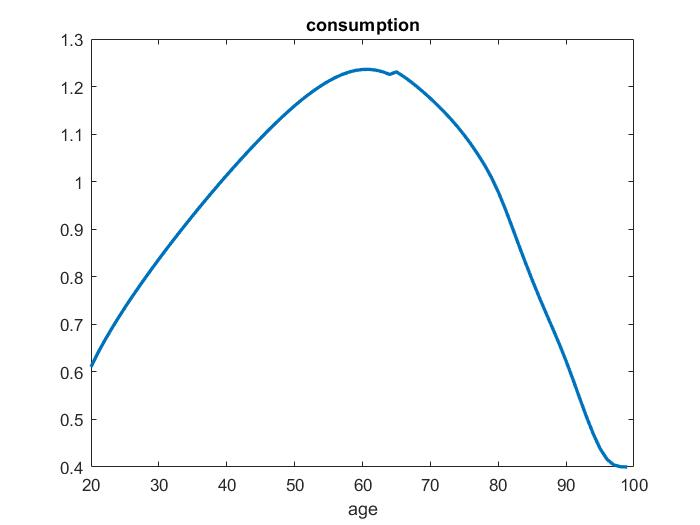
\includegraphics[width=14cm]{Graphs/Figure10} \\
This graph depicts consumption over the life cycle. Similar to assets, consumption increases until a certain point (close to retirement age) and afterwards decreases steadily. \\
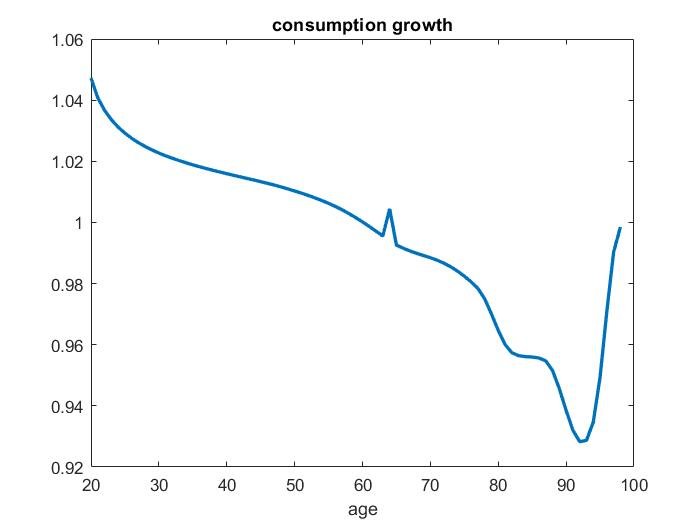
\includegraphics[width=14cm]{Graphs/Figure11} \\
This graph depicts consumption growth. As long as consumption growth is higher that 1, consumption growth is positive, as soon as consumption growth is smaller than 1m consumption growth is negative. Consumption growth is highest when entering the labour market. Afterwards consumption growth gets less and less (except for a small spike close to retirement) and even becomes negative. Only at really high ages (90+), consumption growth increases again. The individual anticipates that he/ she will die at age 100 for sure and wants to consume all his/ her savings before that. \\
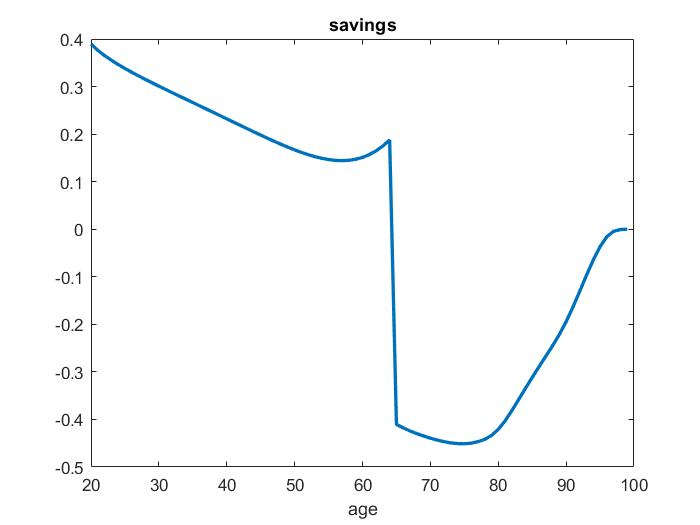
\includegraphics[width=14cm]{Graphs/Figure12} \\
This graph depicts savings (for each period, not aggregate) over the life cycle. Savings are positive until retirement and negativ afterwards. This is in line with the other graphs and theory, suggesting that individuals make precautionary savings to insure againt income risk and old age.\\
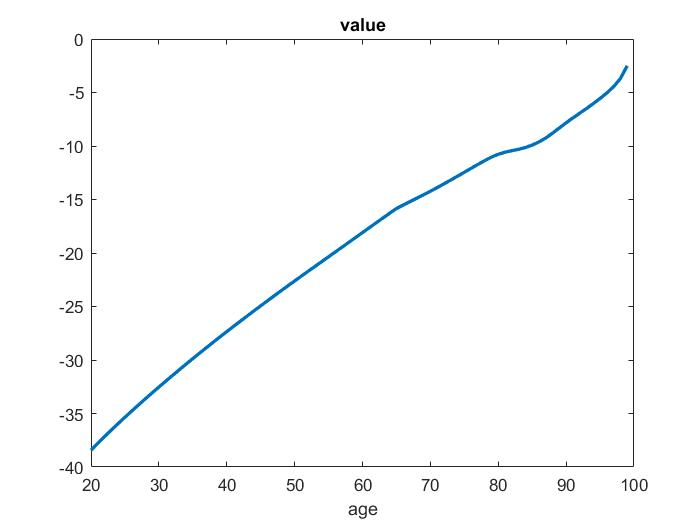
\includegraphics[width=14cm]{Graphs/Figure13} \\
???\\


The function func\_calibr calibrates the model. That is, it specifies the parameters of the model: the interest rate r, $\rho, \beta, \theta,$ the years an induvidual consumes until dying for sure nj, the years an induvidual works jr, the number of grid points nx, the curvature of the grid curv, the scaling factor of saving grid grdfac, the deterministic income components (percentage of net income netw, percentage of net income paid as a pension pens), survival rates, population and fraction living in a specific year, population size pop, number of income states, Markov chain for income shocks (depending on number of income shocks ny, transition probability rhoeta, variance of permanent shock vareta).\\

There is an alternativ Markov chain? \\

The function func\_hh solves the model and returns gridx, gridsav, gridass, cfun, and vfun as outputs. This needs to be compared to a standard implementation of the exogenous grid method (from the lecture). \\

function fv = func\_intp(x,func,xp) \\
This function is a function within func\_hh. It is needed to calculate... \\

function y=func\_extrapol(x1,x2,y1,y2,x)\\
This function is a function within func\_hh. It is needed to calculate a simple linear extrapolation. \\


function [Phi,PhiAss,ass]=fun\_aggr(gridx,gridsav,cfun,gridass)\\
This function calculates the aggregate measures.

function [vals,inds]=basefun(grid\_x,x,nx)\\
This subroutine returns the values and the indices of the two basis functions that are positive on a given x in the grid\_x. It is needed to calculate the aggregate measures. \\

function [labinclife,inclife,asslife,conslife,vallife] = lcprofile(Phi,gridass,cfun,vfun)\\
This function calculates the life cycle profiles.\\

function [pini,pi,gridy]=mchain(rhoeta,epsil)\\
This function defines the Markov chain (transition probabilities and inital distributions). \\

function u = U(c)\\
This small function simply calculates the utility. \\

function muc=MUc(c)\\
This small function simply calculates the marginal utility. \\

function invut=invut(marg)\\
This function inverts untility. This is needed for...\\

function grd = makegrid(x1,x2,n,c) \\
This function makes curved grid according to curvature parameter c. \\

\subsection*{Compare the solution procedure in \purl{func_hh} to a standard implementation of the exogenous grid method}

\subsection*{Implement the standard method of exogenous grid points by working with an exogenous grid for cash-on-hand x}

\subsection*{Implement a standard value function iteration}

\subsection*{Look at \purl{func_aggr}}

\subsection*{Solve the model under the following three alternative settings:}

\begin{enumerate}
\item
\item
\item
\end{enumerate}

\section*{Problem 2: Calibration}

\section*{Problem 3: Analysis}

\section*{Problem 4: Summary of De Nardi (2004)}
Since the distribution of wealth is much more concentrated than the distribution of (labour) earnings, De Nardi (2004) estimates a quantitative, general equilibrium, incomplete markets, overlapping-generations model to match this observation from the data. In doing so, the author links parents and children by accidental as well as voluntary bequests - but not by inter vivo transfers - and allows children to inherit some of their parents' productivity. Further, she calibrates the model to match important features of, first, the data of the U.S. and, second, the data of Sweden. Both countries have different wealth distribitions even though their Gini coefficients are relatively similar. This paper's framework makes it possible for intergenerational links to induce saving behaviour that generates a more concentrated distribution of wealth than that of earnings due to allowing two different saving motives: self-insurance against labour earnings shocks and life-span risk, i.e. saving for retirement, which both can be seen as precautionary motives, and the preference to leave bequests to their offspring, which is an altruistic motive.
\\
De Nardi finds that saving for precautionary purposes and saving for retirement are the primary factors for wealth accumulation at the lower tail of the distribution, while saving to leave bequests significantly affects the shape of the upper tail.

\end{document}
